\chapter{Theoretische Grundlagen}
\label{ch:fundamentals}
Dieses Kapitel stellt dem Leser benötigtes Basiswissen zur Verfügung. Es wird ein grundlegendes Wissen zu den Themenbereichen \ac{DLT} und \ac{IOT} vermittelt und auf weitere Informationsquellen verwiesen, welche tiefergehende Informationen bereitstellen.

%
% Section: DLT
%
\section{Distributed Ledger Technologies}
\label{sec:fundamentals:dlt}
Die Begriffe Blockchain und Distributed Ledger Technology (kurz: \ac{DLT}) werden häufig synonym verwendet\footnote{In dieser Arbeit werden die Begriffe ebenfalls synonym verwendet, andernfalls wird explizit darauf hingewiesen.}, wobei es sich bei Blockchain um eine Unterklasse von \ac{DLT} handelt \cite{mastering2017}. Grundsätzlich werden Daten in Blockchains zu Blöcken zusammengefasst und mittels Hashketten in eine feste Reihenfolge gebracht. \acp{DLT} nutzen darüber hinaus andere Strukturen als Blöcke, indem sie Daten beispielsweise durch Bäume oder Graphen anordnen.\\

\begin{figure}[h]
 \centering
 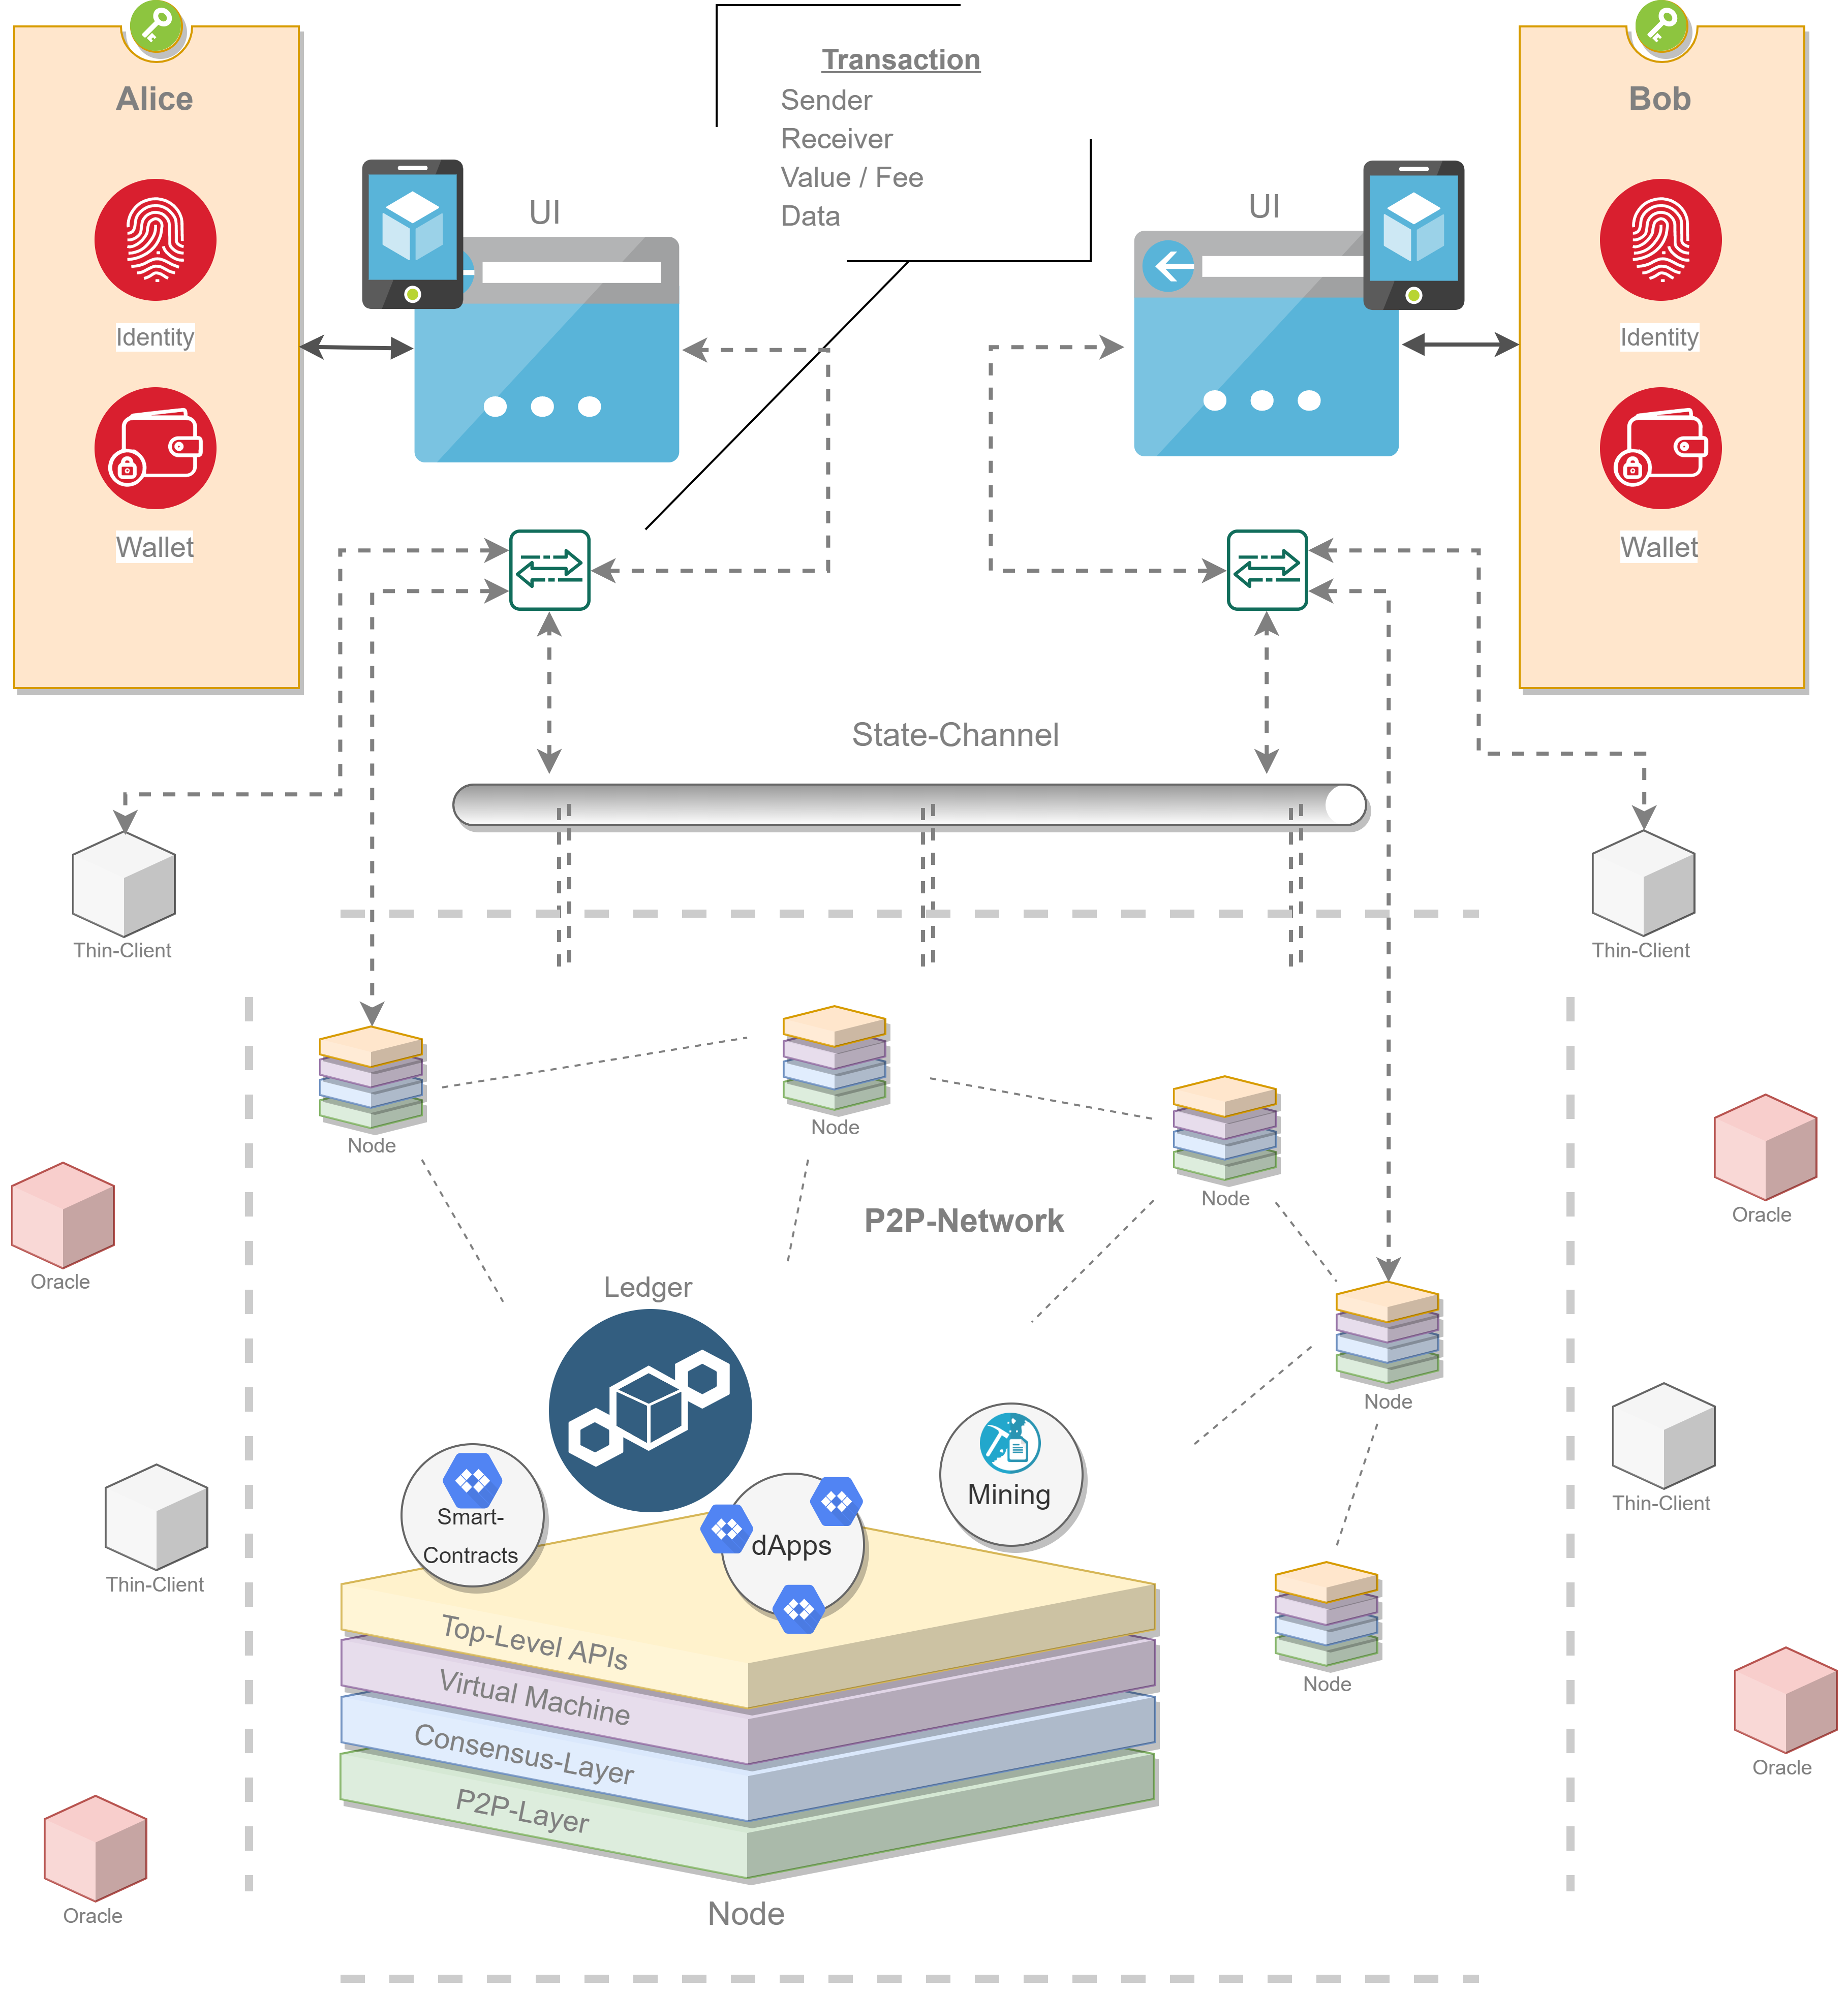
\includegraphics[width=1.0\textwidth]{gfx/Overview-DLT.png}
 \caption{Bestandteile von DLTs}
 \label{fig:chapter02:overview-dlt}
\end{figure}

Abbildung \ref{fig:chapter02:overview-dlt} zeigt die Bestandteile einer \ac{DLT} auf. Diese werden im Folgenden detailliert beschrieben und erklärt.\\
Es handelt sich bei \acp{DLT} um dezentrale \ac{P2P}-Netzwerke, in denen Knoten (engl.: Nodes) Daten dezentral speichern, einen Konsens-Mechanismus zur Synchronisierung einsetzen und asymmetrische Verschlüsselungsverfahren zur Integrität und Absicherung des Systems nutzen. \cite{DLT2016}\\
Hauptbestandteil eines Distributed Ledgers ist der Ledger selbst (deutsch: Kassenbuch), der eine Historie aller erfolgten Transaktionen speichert. Eine Transaktion stellt eine Wert- oder Informationsübertragung zwischen Entitäten dar. Sie beinhaltet einen Sender, einen Empfänger und eine Anzahl Einheiten, die versendet werden sollen. Je nach Implementierung können weitere Inhalte wie zum Beispiel Nutzdaten oder Software-Code dazukommen. Dieser Code, auch Smart-Contract genannt, wird in einer separierten Laufzeitumgebung (Virtual Machine) ausgeführt. Durch das Zusammenspiel mehrerer Smart-Contracts ist man in der Lage, ganze Anwendungen onchain auszuführen; hierbei spricht man von sogenannten \acp{DApp}.\\
Smart-Contracts können nur auf den internen (onchain) State des Ledgers zuzugreifen. Werden darüber hinaus weitere (offchain) Informationen benötigt\footnote{Beispiele hierfür können Wetterdaten, Aktien- und Wechselkurse oder Lottozahlen sein}, so können diese durch sogenannte Oracles an den Smart-Contract übermittelt werden. Diese handeln als 'Trusted Data Provider', da die bereitgestellten Informationen nicht validiert werden können. \cite{ORACLE2019}\\
Transaktionen, die durch Smart-Contracts, \acp{DApp} oder Benutzer ausgeführt werden, müssen von Nodes im Netzwerk validiert werden, bevor sie dem Ledger hinzugefügt werden können. Dazu werden diese durch komplexe Berechnungen zusammengefasst (Mining), dem lokalen Ledger hinzugefügt und anschließend an andere Knoten versendet.\\
Das Konsensprotokoll definiert die Regeln, wann ein Block hinzugefügt werden darf, welche Eigenschaften dieser erfüllen muss und ob das Mining korrekt durchgeführt wurde. Dürfen beliebige Nodes am Konsens teilnehmen, so spricht man von einer Permissionless Blockchain; sind nur priviligierte Nodes befähigt, am Konsens teilzunehmen, handelt es sich um eine Permissioned Blockchain. Darüber hinaus lassen sich Blockchain-Netzwerke klassifizieren, ob Transaktionen und Blöcke öffentlich erreichbar und lesbar sind (Public Blockchain) oder ob auch hier Restriktionen vorliegen (Private Blockchain).\\
Besondere Anforderungen, wie möglichst niedrige Transaktionskosten, eine hohe Transaktiongeschwindigkeit, ein eingeschränkter Wirkungskreis der Anwendung oder Beschränkungen durch das Geschäftsmodell, sind einige Beispiele für die Zulassungsbeschränkung und beschränkte Teilnahme am Konsensverfahren; je nach den gegebenen Anforderungen müssen Blockchain-Protokolle für den jeweiligen Anwendungsfall gewählt oder angepasst werden. Alle Knoten, die dem Konsens-Protokoll folgen und eingehende Blöcke nach diesem Protokoll validieren, heißen Full-Nodes. Daneben existieren sogenannte Light-Clients (oft auch Thin-Clients), die nur Teile des Ledgers vorhalten und meist nur die Block-Header auf Validität überprüfen. Light-Clients sind genauso wie Oracles nicht Teil des \ac{P2P}-Netzwerkes, sondern greifen mittels \ac{API} auf die Nodes zu.\\
Möchte ein Benutzer (in Abbildung \ref{fig:chapter02:overview-dlt} durch Alice und Bob dargestellt) mit der Blockchain kommunizieren oder diese als Kommunikationsmedium nutzen, so geschieht dies ebenfalls über entsprechende \acp{API}. Über eine grafische Benutzeroberfläche können Benutzer meist per Browser oder Smartphone Transaktionen auslösen und diese über das Blockchain-Netzwerk verschicken. Jeder Benutzer besitzt eine Wallet, die aus einem öffentlichen und einem privaten Schlüssel besteht (Public / Private Key). Der Public-Key gleicht der Kontoaddresse eines Bankkontos, der dazugehörige Private-Key der PIN-Nummer. Damit besitzt jeder Nutzer eine eindeutige Identität.\\
Möchte Alice eine Transaktion im Wert von 10 € an Bob senden, so kann sie dies auf unterschiedlichen Wegen tun. Zunächst einmal kann sie die gewünschten Informationen auf ihrem Smartphone mittels einer Wallet-App eingeben und per Knopfdruck an das Blockchain-Netzwerk übermitteln. Diese wird dort über die entsprechende \ac{API} empfangen, verarbeitet und im Ledger persistiert. Bob kann ebenfalls mittels seiner Smartphone-App verfolgen, wann sich sein Kontostand ändert und wer eine Transaktion an seine Adresse gesendet hat.\\
Eine alternative Lösung hierzu wäre der Einsatz von sogenannten State-Channels. Diese können Alice und Bob dazu nutzen, beliebig viele Transaktionen untereinander offchain auszutauschen und lediglich die endgültige Bilanz aller untereinander ausgetauschten Transaktionen onchain in den Ledger zu übertragen.\\
Die Vor- und Nachteile beider Varianten sowie die in diesem Abschnitt aufgezeigten Fachbegriffe werden im weiteren Verlauf genauer erläutert.



\subsection{Konsensprotokolle}
\label{subsec:fundamentals:dlt:consensus}
Transaktionen und Daten müssen über das Gesamtsystem hinweg konsistent sein. Um dies und die Integrität der Daten zu gewährleisten, bedarf es eines Mechanismus, welcher sicherstellt, dass alle Knoten die gleichen Daten halten.\\
Solche Mechanismen werden durch Konsensprotokolle beschrieben: Es handlet sich dabei um ein Protokoll, welches Regeln definiert, wie und welche Daten gespeichert und welche verworfen werden. Im Folgenden werden einige bekannte Konsensverfahren genannt und kurz vorgestellt.
\begin{description}
  \item[Proof-of-Work (PoW)] Transaktionen werden zu Blöcken zusammengefasst. Diese Blöcke werden durch das Lösen eines kryptografischen Puzzles (Mining) wie zum Beispiel die Ermittlung eines Hashwertes abgesichert. Ein Knoten, der einen Block dem Ledger hinzufügen möchte, muss zuerst eine zufallsbasierte Berechnung durchführen, um dem Netzwerk die Validität zu beweisen. Andere Knoten können mit sehr wenig Aufwand überprüfen, ob die Berechnung korrekt war und der Knoten ehrlich gehandelt hat. Dieses Konsensverfahren ist meist mit einem hohen Stromverbrauch verbunden, da die zeitaufwändige Berechnung viele Ressourcen benötigt. \cite{Salimitari2018ASO}
  \item[Proof-of-Stake (PoS)] Unter der Annahme, dass Knoten mit hoher finanzieller Beteiligung (Stake) ehrlich agieren, um der Plattform nicht zu schaden und ihre finanziellen Mittel nicht zu gefährden, werden diese bei der Auswahl bevorzugt, eine Transaktion dem Ledger hinzuzufügen. Dieses Verfahren ist deutlich stromsparender als PoW, allerdings durch die Miteinbeziehung des Vermögens auch ungerechter im direkten Vergleich. \cite{Salimitari2018ASO}
  \item[Delegated-Proof-of-Stake (dPoS)] Dieses Verfahren ergänzt PoS um ein Delegierten-System, was die Anzahl an potentiellen Konsensknoten stark einschränkt und damit die Performance erhöht: Statt einen Konsens zwischen allen beteiligten Knoten zu finden, werden delegierte Knoten gewählt, die stellvertretend für andere über die Richtigkeit der Transaktionen abstimmen. Durch die geringere Teilnehmeranzahl am Konsens und die damit einhergehende, geringe Anzahl an benötigten Nachrichten, um zu einem gemeinsamen Ergebnis zu gelangen, wird die Performanz erhöht. Knoten, die bösartig handeln, können aus dem Konsens herausgewählt werden. \cite{Salimitari2018ASO}
  \item[Practical Byzantine Fault Tolerance (PBFT)] Um in der Lage zu sein, bis zu einem Drittel an bösartigen Knoten handhaben zu können ('The Byzantine generals problem', siehe \cite{byzantine2019}), müssen alle Knoten des Gesamtsystems bekannt sein. Dieses Verfahren löst das Konsensproblem, indem der Konsens in Runden eingeteilt wird und jede Runde Transaktionen in den Ledger übernommen werden. Indem die Knoten untereinander ihre Validierungsergebnisse austauschen, können ein Mehrheitsentscheid durchgeführt und damit die korrekten Transaktionen identifiziert werden. \cite{Salimitari2018ASO}
  \item[Proof-of-Authority (PoA)] Dieses Verfahren wird meist in privaten und Permissioned Blockchains eingesetzt. Die Konsensknoten sind fest definiert und fungieren als Autorität des Gesamtsystems. Da kein Mining existiert, können Transaktionskosten minimal gehalten werden und das System kann aufgrund des einfachen Aufbaus des Konsens sehr gut skalieren. \cite{Salimitari2018ASO}
\end{description}
Detailliertere Informationen sowie weitere Konsensverfahren können \cite{overview2017} und \cite{consensusIOT2018} entnommen werden.

\subsection{Smart-Contracts}
\label{subsec:fundamentals:dlt:smartcontracts}
Bei Smart-Contracts handelt es sich um Software-Code, der auf der Blockchain (onchain) auf allen Knoten ausgeführt wird und eine Zustandsänderung meist in Form von ausgehenden Transaktionen zur Folge hat. Smart-Contracts werden in einer abgeschirmten Laufzeit-Umgebung (engl.: Runtime-Environment) ausgeführt; im Falle von Ethereum spricht man von der \ac{EVM}. \cite{smartcontracts2017}\\
Um auf Daten und Informationen außerhalb des Blockchain-Netzwerkes zugreifen zu können, bedienen sich Smart-Contracts sogenannter Oracle-Services. Dabei handelt es sich um Informationsanbieter (Trusted Data Provider), die zum Beispiel Wetterdaten, Lottozahlen oder Nahverkehrsinformationen an einen Smart-Contract senden, damit dieser, basierend auf den empfangenen Daten, seine Logik ausführen und die Daten verarbeiten kann. Der grundlegende Nachteil von Oracle-Services liegt in der Vertrauensfrage: Während eine Blockchain grundsätzlich mittels Konsensverfahrens die Vertrauensfrage beantwortet, obliegt dem Besitzer bzw. Betreiber eines Oracles die Macht über die Richtigkeit der Daten. Dieser Problematik kann durch den Einsatz mehrerer, mittels eines separat implementierten Konsenses abgestimmter Oracle-Services entgegengewirkt werden. \cite{ORACLE2019}\\
Mit dem Software-Code von Smart-Contracts können komplexe Logiken, so auch Vertragslogiken von Kauf- oder Mietverträgen, abgebildet und automatisiert abgearbeitet werden. Bei der Umsetzung und Automatisierung von juristischen Verträgen ist das jeweils geltende Recht eines Landes zu beachten: Die Form und der Aufbau sowie der abzubildende Inhalt eines Vertrages müssen gewissen Normen entsprechen und alle benötigten Informationen enthalten, damit ein Vertrag rechtskräftig ist. \cite{smartcontracts2017}

\subsection{Dezentrale Apps (DApps)}
\label{subsec:fundamentals:dlt:dapps}
Eine \ac{DApp} ist eine Anwendung, die auf dem Blockchain-Netzwerk dezentral ausgeführt wird. Die Applikationslogik wird dabei durch einen Smart-Contract oder durch den Zusammenschluss mehrerer Smart-Contracts abgebildet \cite{dapps2018}. Eine \ac{DApp} kann demnach - genauso wie ein einzelner Smart-Contract - nicht auf Informationen außerhalb der Blockchain zugreifen; es sei denn, Informationen werden durch Oracles bereitgestellt. Da \acp{DApp} als solche keine dedizierte Benutzerschnittstelle besitzen, sondern lediglich über Blockchain-typische \acp{API} erreichbar sind, trifft man \acp{DApp} meist in Verbindung mit einer Web-Applikation an, die dem Benutzer die Interaktion ermöglicht \cite{DAPPS2016}.\\
Da eine Datenhaltung onchain sehr kostenintensiv ist, bietet es sich an, diese offchain zu speichern. Im Sinne einer dezentralen Anwendung bietet sich hierbei der Einsatz von Technologien wie \ac{IPFS}\footnote{Dezentrales, verteiltes Dateisystem, basierend auf einem \ac{P2P}-Netz. Dateien werden versioniert und sind mittels Fingerprint(Hashing) eindeutig identifizierbar.} an. Daten können dezentral und kostengünstig außerhalb des Blockchain-Netzwerkes aufbewahrt, allerdings onchain eindeutig referenziert werden.\\
In Abbildung \ref{fig:chapter02:overview-dapp} wird ein beispielhafter Aufbau einer \ac{DApp} aufgezeigt.

\begin{figure}[h]
 \centering
 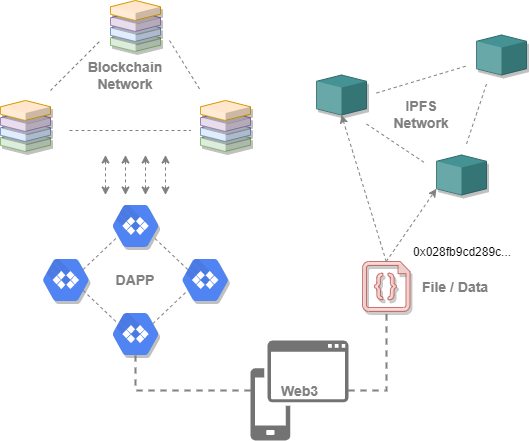
\includegraphics[width=1.0\textwidth]{gfx/Overview-DAPP.png}
 \caption{Aufbau von DApps}
 \label{fig:chapter02:overview-dapp}
\end{figure}

\acp{DApp} haben den Vorteil, dass sie alle Stärken der Blockchain besitzen: Sie sind dezentral organisiert, manipulations- und ausfallsicher \cite{DAPPS2016}. Durch Kryptowährungen wie Ether oder andere ERC20-Token können Zahlungsabwicklung nativ integriert werden. Auf der anderen Seite sind zum Beispiel Performanz und Ausführungskosten an die Kapazitäten und Eigenschaften des Blockchain-Netzwerkes gebunden. Damit sind zeitkritische oder Performanz-lastige Anwendungen nicht oder nur in Ausnahmefällen für eine Implementierung auf einer Blockchain geeignet.

\subsection{Klassifizierung von Blockchains}
\label{subsec:fundamentals:dlt:classification}
Blockchains können nach \citeauthor{overview2017} (vgl. \citetitle{overview2017}, \cite{overview2017}) klassifiziert werden, indem man die Sichtbarkeit von Informationen sowie die aktive Teilnahme von Netzwerkknoten am Konsensmechanismus betrachtet. Ist die Blockchain öffentlich erreichbar und können Transaktionen und Blöcke von beliebigen Knoten eingesehen werden, so handelt es sich um eine öffentliche (Public) Blockchain. Ist der Zugang zum Blockchain-Netzwerk beschränkt und können nur berechtigte Knoten Transaktionen und Blöcke einsehen, so spricht man von einer privaten (Private) Blockchain. Eine besondere Form der Private-Blockchain ist die Konsortial-Blockchain; hierbei handelt es sich oftmals um einen Zusammenschluss mehrerer Entitäten, meist Unternehmen, welche die Zugangsbeschränkung zur Blockchain verwalten. Zur besseren Verständlichkeit können Private- und Public-Blockchains analog zu Intranet (firmenintern) und Internet (weltweit für jeden zugänglich) gesehen werden.\\
Darüber hinaus lassen sich Blockchains laut \citeauthor{overview2017} über die Teilnahme am Konsensprotokoll klassifizieren: Ist jeder Netzwerkknoten, der die Blockchain erreichen und damit Informationen einsehen kann (unabhängig von Public oder Private), berechtigt, am Konsensverfahren teilzunehmen, so spricht man von einer beschränkungslosen (Permissionless) Blockchain. Ist das Konsensverfahren auf priviligierte Knoten beschränkt, so handelt es sich um eine zugangsbeschränkte (Permissioned) Blockchain. Die vorgestellten Klassifizierungen in Public, Private, Permissioned und Permissionless lassen sich darüber hinaus kombinieren, wodurch es vier mögliche Arten von Blockchains gibt. Abbildung \ref{fig:chapter02:taxonomy} stellt diese schematisch dar und listet dazu einige bekannte Umsetzungen auf.

\begin{figure}[htbp]
 \centering
 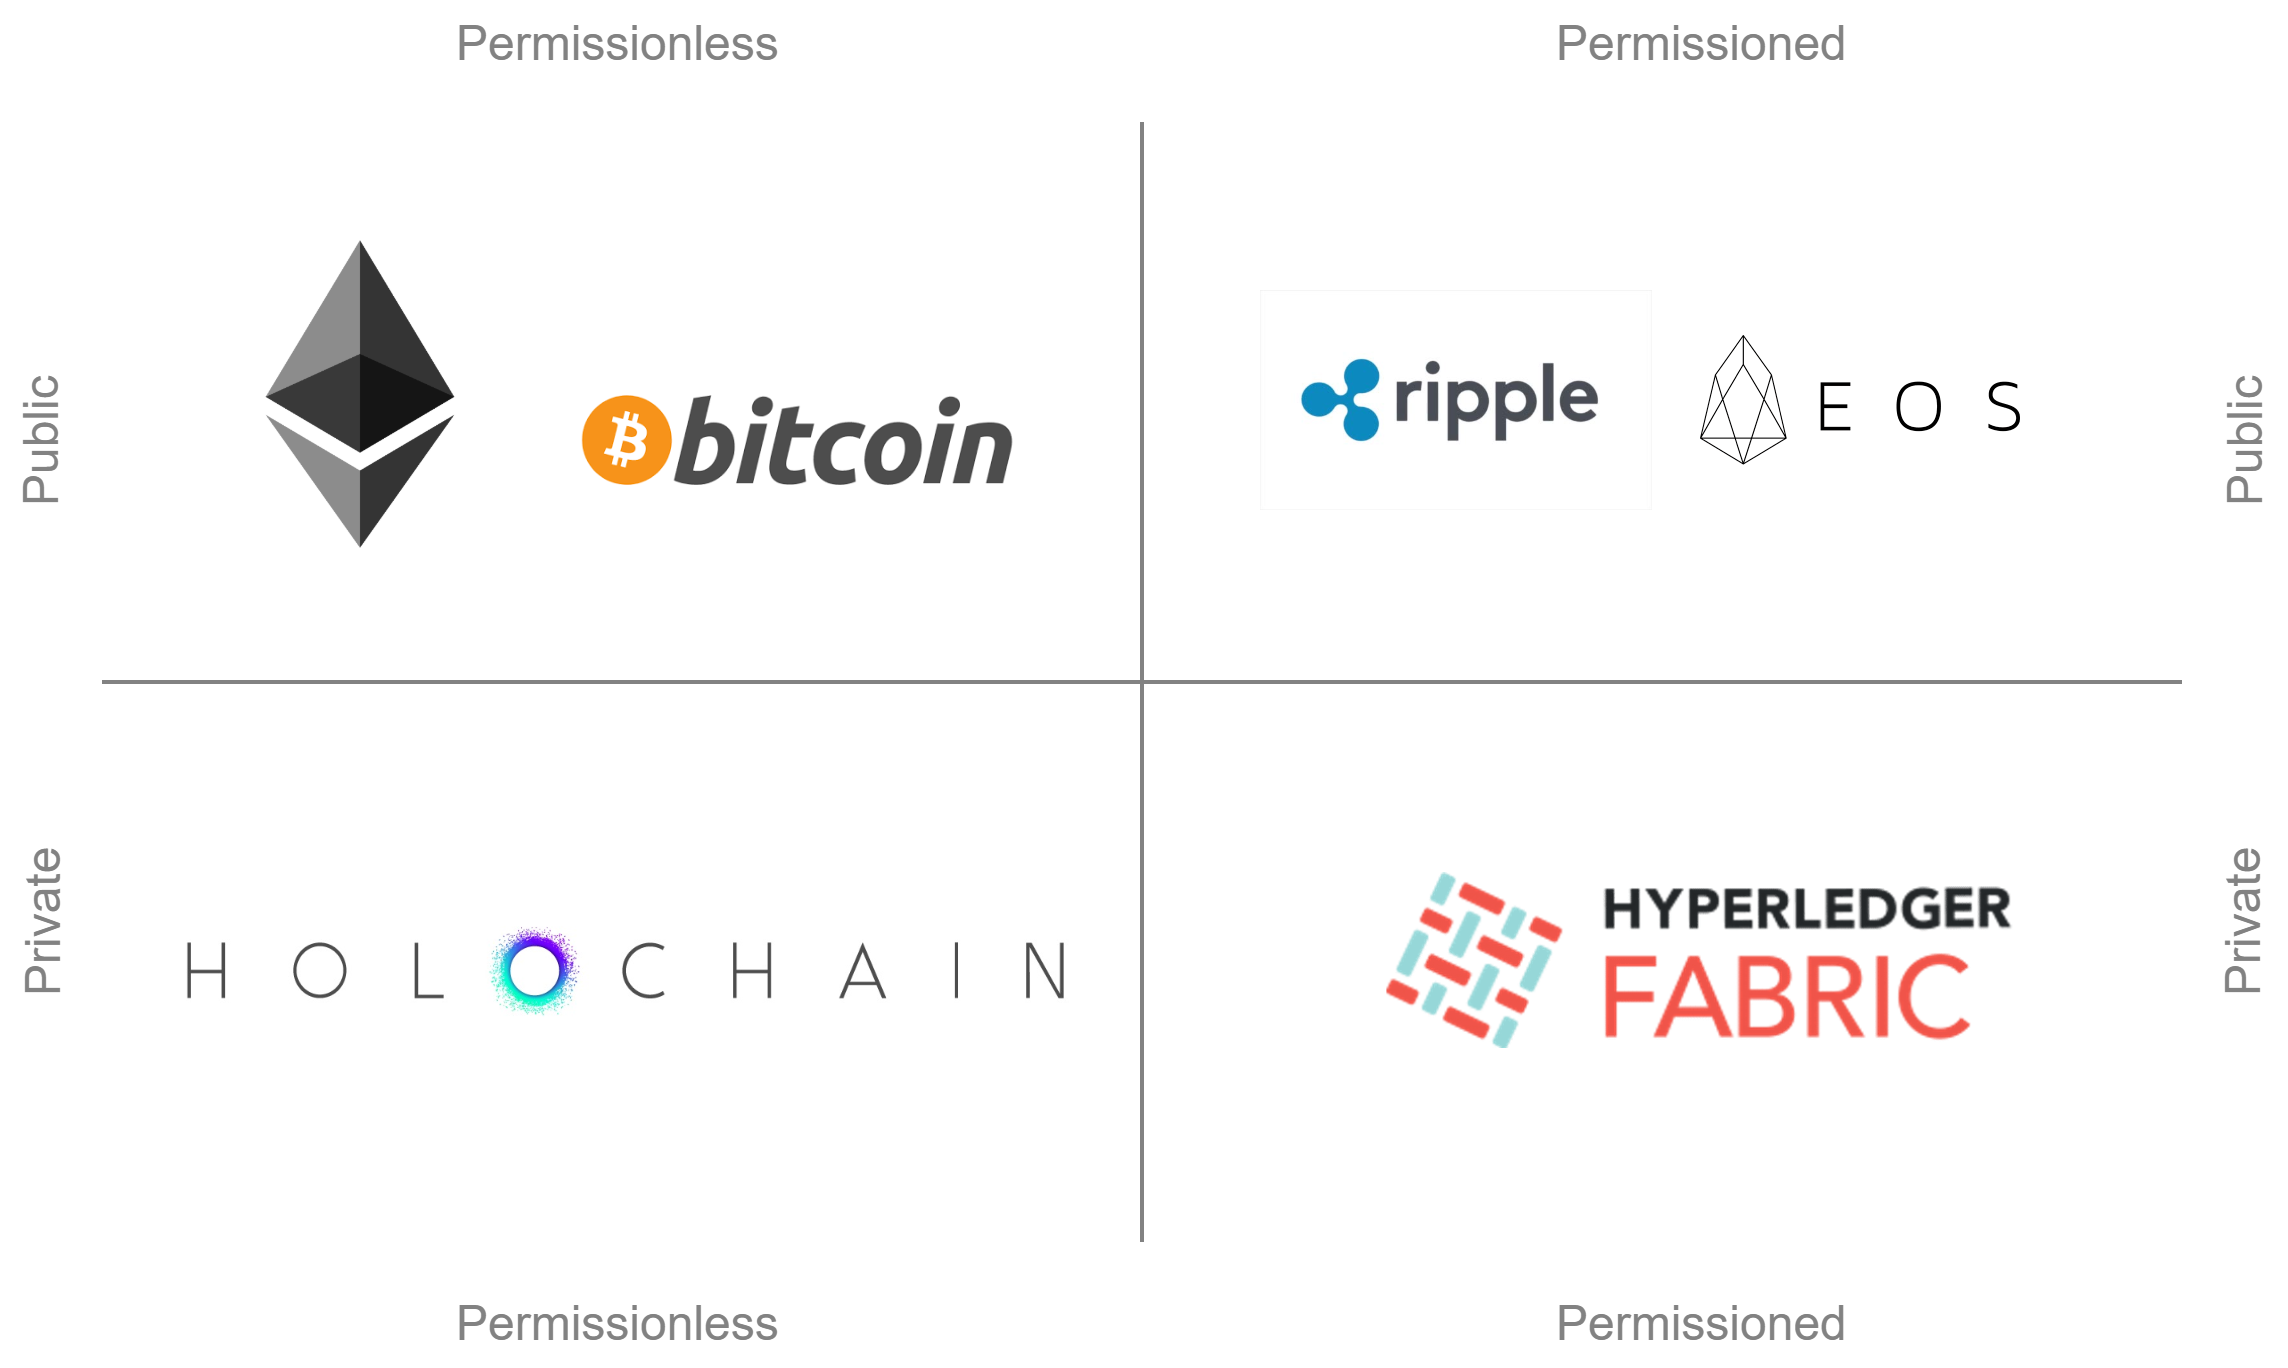
\includegraphics[width=0.8\textwidth]{gfx/taxonomy.png}
 \caption{Taxonomie von Blockchains (vgl. \cite{daniels2018})}
 \label{fig:chapter02:taxonomy}
\end{figure}

Die bekanntesten Vertreter Bitcoin und Ethereum sind öffentliche und beschränkungslose Blockchains, an denen jeder teilnehmen kann und alle Daten öffentlich einsehbar sind. Die Klassifizierung ergibt sich als logische Konsequenz aus besonderen Anforderungen an die Blockchain: So können Transaktionskosten, Transaktiongeschwindigkeiten, der Wirkungskreis der Anwendung oder das Geschäftsmodell Argumente für die Zulassungsbeschränkung und beschränkte Teilnahme am Konsensverfahren sein. Daraus resultiert, dass Blockchain-Protokolle je nach gegebenen Anforderungen des Anwendungsfalls ausgewählt und abgewägt werden müssen.

\subsection{Wallets}
\label{subsec:fundamentals:dlt:wallets}
%http://groups.csail.mit.edu/cis/crypto/classes/6.857/papers/secret-shamir.pdf
%https://hackernoon.com/shamir-secret-sharing-vs-multi-sig-124a42bc1662
%https://www.binance.vision/de/security/threshold-signatures-explained
%https://medium.com/zengo/threshold-signatures-private-key-the-next-generation-f27b30793b
Einer Wallet ist ein Kontostand zugeordnet, sie besteht aus einem privaten Schlüssel (Private Key) und dem dazugehörigen öffentlichen Schlüssel (Public Key) und hat einen eindeutigen Eigentümer - den Besitzer des Private Keys. Der Public Key ist (in den meisten Fällen) die öffentliche Adresse, die für Transaktionen genutzt wird und entspricht in etwa einer Kontonummer einer Bank. Der Private Key fungiert als PIN-Nummer und ist nur dem Eigentümer der Wallet bekannt.\\
Multisignatur-Wallets sind Wallets, auf deren Inhalt nur durch den Einsatz mehrerer Private Keys zugegriffen werden kann. Dabei wird ein Multisignatur-Wallet von \textit{n} Schlüsseln erzeugt. Um auf den Inhalt zugreifen zu können, bedarf es der Signaturen von \textit{t von n} Schlüsseln. Dadurch können verschiedene Anwendungsfälle wie zum Beispiel Treuhandkonten (2 von 3), Zwei-Wege-Authentifizierungen (2 von 2) und viele weitere abgedeckt werden. \cite{multisig2018}\\
Multisignatur-Wallets können entweder Teil des Blockchain-Protokolls sein und damit nativ unterstützt oder beispielsweise durch die Umsetzung mittels Smart-Contract realisiert werden. Letzteres ist dabei denkbar einfach: Es handelt sich um Code, der erst dann eine Transaktion ausführt, wenn mit \textit{t von n} der hinterlegten Schlüssel unterschrieben wurde. Die Höhe von \textit{t} und \textit{n} ist im Code festgelegt.

% Die Idee von Multisignatur-Wallets geht zurück auf das Shamir Secret Sharing Verfahren, welches im Folgenden kurz dargelegt wird:\\
% \textbf{\textcolor{red}{todo}}\\
% Ein großer Nachteil des Shamir Secret Sharing Verfahrens ist, dass bei der initialen Schlüsselgenerierung und bei der Entschlüsselung der vollständige private Schlüssel zusammengesetzt und damit an einem geografischen Ort vorhanden ist. Dies bietet ein gewisses Angriffspotential. Eine Weiterentwicklung des Shamir Secret Sharing Verfahrens ist das Schwellenwert-Signaturschema (engl. Threshold Signature Scheme, TSS), welches sich der \ac{MPC} bedient, wodurch der private Schlüssel niemals vollständig an einem Ort vorhanden ist. Um gemeinsam zu signieren oder entschlüsseln zu können, müssen alle beteiligten Parteien zeitlich synchron an dem Prozess teilnehmen. Das Verfahren wird im Folgenden kurz erläutert. Tiefergehende Informationen können X oder Y entnommen werden.\\
% \textbf{\textcolor{red}{todo}}
% Grundsätzlich verfolgen alle drei Verfahren - das Multisignatur-Wallet, das Shamir Secret Sharing Verfahren und das Schwellenwert-Signaturschema - das gleiche Ziel: Ein Geheimnis, wie zum Beispiel ein Private Key, wird auf mehrere Instanzen verteilt. Diese müssen an einem Ort zusammenkommen und ihre Teilgeheimnisse zusammenfügen, um Daten entschlüsseln oder signieren zu können. Dabei unterscheiden sich die Verfahren unter Anderem in der zeitlichen Synchronität und geografische Lage des Schlüssels.

\subsection{Dezentrale Identitäten}
\label{subsec:fundamentals:dlt:did}
Eine Identität zeichnet sich durch eine Menge von Informationen, Daten und Eigenschaften aus, die diese eindeutig identifizieren. Nur der Inhaber einer Identität kann mit dieser auch agieren, da er der einzige ist, der Zugriff auf die geschützten Informationen hat, die die Identität des Inhabers bestätigen. Diese können zum Beispiel ein Passwort, eine Geburtsurkunde, ein Fingerabdruck oder Ähnliches sein.\\
Eine dezentrale Identität ist laut \cite{DID2007} eine neuartige Technologie, die es dem Inhaber einer solchen erlaubt, seine Identität digital, dezentral und sicher durch den Einsatz asymmetrischer Verschlüsselung selbst zu verwalten. Sie ist kryptografisch verifizierbar und der Inhaber entscheidet selbst, welche Informationen er teilen möchte und welche nicht. Das \ac{W3C} entwickelt aktuell (Stand: Dezember 2019) einen Industrie-Standard, der zur Verifizierung und Authentifizierung persönlicher Informationen vor Dritten im Web 3.0 eingesetzt werden soll und sich derzeit in der Version 1.0 befindet \cite{did2019}. Eine dezentrale Identität besteht aus einer \ac{DID}, welche weltweit einzigartig ist, und einem dazugehörigen DID-Dokument, welches Informationen über den beschriebenen Gegenstand enthält. Die folgenden Beispiele zeigen eine \ac{DID} und ein dazugehöriges DID-Dokument (entnommen aus \cite{did2019}).

\begin{lstlisting}[caption=Beispiel einer DID,label=listing:did]
did:example:123456789abcdefghi
\end{lstlisting}

\begin{lstlisting}[caption=Beispiel eines DID-Dokuments,label=listing:did_document]

{
  "@context": "https://www.w3.org/ns/did/v1",
  "id": "did:example:123456789abcdefghi",
  "authentication": [{

    "id": "did:example:123456789abcdefghi#keys-1",
    "type": "RsaVerificationKey2018",
    "controller": "did:example:123456789abcdefghi",
    "publicKeyPem": "-----BEGIN PUBLIC KEY...END PUBLIC KEY-----\r\n"
  }],
  "service": [{

    "id":"did:example:123456789abcdefghi#vcs",
    "type": "VerifiableCredentialService",
    "serviceEndpoint": "https://example.com/vc/"
  }]
}
\end{lstlisting}

Durch den Einsatz von Blockchain-Technologie können \acp{DID} manipulationssicher, hochverfügbar und für jeden zugänglich gespeichert werden. Die \ac{DID} besteht aus drei Teilen: Zunächst dem Schlüsselwort 'did', welches beschreibt, dass es sich um eine \ac{DID} handelt. Anschließend folgt die DID-Methode (im Beispiel: example), die definiert, wie die \ac{DID} aufzulösen und weitere Informationen zu dieser Identität zu finden sind. Der letzte Teil ist eine ID (vgl. \ref{listing:did}), die für jede Methode einzigartig ist und somit eindeutig ermittelt werden kann.\\
In diesem Kontext existieren sogenannte \acp{VC}, die einer \ac{DID} von vertrauenswürdigen Instanzen ausgestellt werden können. Dabei handelt es sich um verifizierbare Berechtigungsnachweise. Der Aussteller bescheinigt dem Empfänger eine bestimmte Eigenschaft und stellt einen Service-Endpoint zur Verfügung, an dem ein Dritter diesen \ac{VC} verifizieren kann. \cite{did2019}\\
So kann zum Beispiel eine Universität mit ihrer eigenen \ac{DID} 'did:hda:12345' einem Student 'did:test:sebastiankanz' ein \ac{VC} ausstellen, welches Studenten bescheinigt, aktuell an der Universität eingeschrieben zu sein. Möchte sich ein Student nun an der Universitätsbibliothek authentifizieren, so kann er dort das \ac{VC} der Universität vorzeigen und bekommt Zugriff auf die Bibliotheksausleihe. Die Bibliothek kann das \ac{VC} verifizieren, indem er unter der Methode 'hda' die Universität identifiziert und anschließend die Signaturen überprüft.


\subsection{State-Channel}
\label{subsec:fundamentals:dlt:scaling}
%https://hackernoon.com/difference-between-sidechains-and-state-channels-2f5dfbd10707
Blockchains\footnote{Hinweis: Es handelt sich bei dieser Betrachtung primär um Public Blockchains unabhängig vom eingesetzten Konsensverfahrens. Das Skalierungsproblem kann allein durch die Beschränkung auf eine Private Blockchain meist gelöst werden.} gehen aufgrund ihrer Beschaffenheit einen Kompromiss ein. Durch das Konsensprotokoll ist unabhängig von Blockgröße und Netzwerkkapazität ein natürliches Limit gegeben: Das Bitcoin-Netzwerk ist beispielsweise durch die komplexe Berechnung von \ac{PoW} auf eine Blockzeit von 10 Minuten beschränkt. Ist die Blockgröße sehr klein, können Blöcke sehr schnell über das Netzwerk propagiert, allerdings nur wenige Transaktionen auf einmal übertragen werden. Ist die Blockgröße sehr groß, ist es sehr schwer für Knoten, sich zu synchronisieren. Dafür können mehr Transaktionen auf einmal übertragen werden.\\
Durch diese Limitierung von Blockgröße und Blockdauer sind im Fall von Bitcoin derzeit (Stand 01/2020) durchschnittlich etwa 7 Transaktionen pro Sekunde möglich \cite{Macdonald2017}. Andere Implementierungen nutzen gegebenenfalls andere Konsensmechanismen und andere Parameter, allerdings liegen auch dort natürliche Schranken vor. Es wird deutlich, dass mit steigenden Anforderungen vor allem an die Transaktionsverarbeitung pro Zeitintervall (meistens \ac{TPS}) eine verbesserte Performanz und neue Lösungsansätze erforderlich werden. Es wird eine Lösung für die schlechte Skalierung von Blockchains gesucht. \cite{Macdonald2017}\\
Als eine mögliche Antwort auf das Skalierungsproblem von Blockchains werden sogenannte State-Channels entwickelt. Ziel ist es dabei, jegliche Arten von Status-ändernden Operationen off-chain zu prozessieren, die typischerweise auf der Blockchain ausgeführt und onchain gespeichert werden. Dadurch können die Anzahl an Zugriffen auf die Blockchain sowie die Anzahl an Transaktionen verringert und gleichzeitig die Interaktionszeit zwischen einzelnen Parteien verbessert werden. Im Kontext von Zahlungen (Payments) werden dadurch sogenannte Micro-Payments ermöglicht; bei State-Channels, die sich auf die Zahlungsabwicklung beschränken, spricht man von Payment-Channels. Diese können schneller und günstiger als normale Transaktionen erfolgen. Die Kosten solcher Micro-Payments können sehr gering gehalten werden, da nicht alle Transaktionen auf der Blockchain gespeichert werden. \cite{Coleman2018}\\
Die Grundidee dabei ist folgende: Alice und Bob reservieren einen Teil ihres Vermögens auf der Blockchain, sodass sie vorerst nicht darüber verfügen können und eröffnen einen Payment-Channel zueinander. Diese Transaktion, also das Eröffnen des Payment-Channels, wird auf der Blockchain gespeichert. Das Volumen des Channels, also das Vermögen, dass Alice und Bob nun zwischen einander austauschen können, entspricht der Summe der reservierten Vermögen. Ihr gewünschtes Vermögen, welches für den Payment-Channel reserviert werden soll, kann entweder mittels Multisignatur-Wallet (vgl. Kap. \ref{subsec:fundamentals:dlt:wallets}) oder Smart-Contract (vgl. Kap. \ref{subsec:fundamentals:dlt:smartcontracts}) reserviert werden. Alice und Bob haben nun einen State von jeweils 50 Euro. Anschließend können sich beide signierte off-chain Transaktionen schicken (also nicht über das Blockchain-Netzwerk). Diese Transaktionen enthalten den neuen State: Überweist Bob 10 Euro an Alice, so ändert sich der State von Alice von 50 Euro auf 60 Euro. Schickt Bob erneut eine Transaktion von 10 Euro, so ändert sich der State von Alice auf 70 Euro. Diesen Vorgang können beide nun solange wiederholen, wie sie möchten; solange sie sich in dem Volumen von 100 Euro bewegen. Zum Schließen eines Channels senden Alice oder Bob eine Transaktion an das Blockchain-Netzwerk, welche den finalen State enthält (im Beispiel hat Alice 70 Euro und Bob 30 Euro). Für theoretisch unendlich viele Transaktionen zwischen Alice und Bob müssen lediglich die eröffnende und die schließende Transaktion des Payment-Channels onchain gespeichert werden.\\
%https://busy.org/@bit-news/scalability-solutions-part-1
Einen weiteren, großen Vorteil liefert die durch den State-Channel ermöglichte Asynchronität von Transaktionen. Befinden sich Teilnehmer nicht im Blockchain-Netzwerk (zum Beispiel durch Konnektivitätsprobleme), so können keine Transaktionen durchgeführt werden. Hängen reale Aktionen wie zum Beispiel das Öffnen einer Schranke oder das Prozessieren einer Aktion mit einer Blockchain-Statusaktualisierung zusammen, so würde bei Konnektivitätsverlust der reale Prozess zum Stillstand kommen, bis die Verbindung wiederhergestellt wird. State-Channel könnten hierbei eingesetzt werden, um eine redundante Verbindung zu schaffen, die auch bei Nicht-Erreichbarkeit der Blockchain genutzt werden könnte. Einige Beispiel-Implementierungen von State-Channels sind Bitcoins Lightning Network \cite{Lightning2016}, Ethereums Raiden Network oder die Implementierung von Neo namens Trinity \cite{Trinity2018}.\\
Eine weitere Möglichkeit, Blockchain-Anwendungen zu skalieren, kann durch den Einsatz von Side-Chains \cite{sidechain2019} geschaffen werden. Hierbei handelt es sich um separate Blockchains, die parallel zur Haupt-Blockchain (auch oft Eltern-Blockchain oder Main-Chain genannt) laufen. Um eine Side-Chain zu eröffnen, muss zunächt der Beweis erbracht werden, dass alle Assets, deren Status in der Side-Chain verändert werden sollen, auf der Main-Chain gesperrt oder reserviert sind, sodass der Eigentümer temporär nicht über diese verfügen kann (beispielsweise durch Zero-Knowledge Proofs, siehe \cite{zeroknowledge2020}). Diese gesperrten Assets können anschließend in die Side-Chain transferiert werden. Dort kann der Status verändert werden; beispielsweise kann eine Geld-Transaktion durchgeführt werden. Soll ein Asset zurück auf die Main-Chain transferiert werden, so muss der Beweis erbracht werden, dass dieses Asset auf der Side-Chain gesperrt wurde. Dadurch werden Effekte wie das Double-Spending verhindert.\\
Bei Lösungsansätzen wie State-Channels und Side-Chains spricht man von dem sogenannten Layer-2 Ansätzen: Unter diesem Begriff werden Ansätze verstanden, die nicht direkt auf der Blockchain selbst (Layer-1), sondern auf einem separaten System ausgeführt werden.

\subsection{Blockchain als Kommunikationsprotokoll}
\label{subsec:fundamentals:dlt:protocol}
Das \ac{OSI} Modell gilt seit Mitte der 80er-Jahre als Standard zur Einordnung von Netzwerkprotokollen. Es wurde von der \ac{ISO} entwickelt und besteht aus sieben Schichten (\cite{OSI1980}, \cite{osi2014}):
\begin{description}
  \item[Physical Layer] Die Übertragung des Bit-Datenstroms über ein physikalisches Medium (Hardware) findet auf dieser Ebene statt.
  \item[Data Link Layer] Diese Schicht kapselt Daten in Datenframes; es werden grundlegende Funktionalitäten zur Fehlererkennung und Fehlerbehebung bereitgestellt. Bekannte Protokolle dieser Ebene sind zum Beispiel Ethernet und \ac{ARP}.
  \item[Network Layer] Diese Schicht kapselt Daten in Datenpaketen und implementiert Sequenznummern, Flusskontrolle und Funktionalitäten fürs Routing.
  \item[Transport Layer] Diese Schicht ist zuständig für die Ende-zu-Ende Übermittlung von Daten, die sie vom Session Layer empfängt. Die Daten werden in sogenannte Segmente unterteilt und über das Netzwerk versendet und auf der Empfängerseite ebenfalls von der Transport-Schicht wieder zusammengesetzt.
  \item[Session Layer] Kommunikationskanäle, Sessions genannt, werden auf dieser Schicht geöffnet, geschlossen und verwaltet.
  \item[Presentation Layer] Diese Schicht ist zuständig für Datenkonvertierungen, -kompressionen und stellt Funktionalitäten wie Ver- und Entschlüsselung bereit.
  \item[Application Layer] Diese Schicht stellt die Schnittstelle zum Benutzer dar.
\end{description}

Bei einem dezentralen Netzwerk wie \ac{DLT} liegt es nahe, eine Einordnung in das \ac{OSI} Modell durchzuführen. Dazu werden die verschiedenen Bestandteile eines \acp{DLT} vorgestellt und den Schichten des \ac{OSI} Modells zugeordnet. Die Schichten eins bis drei (Physical, Data Link und Network) werden hierbei nicht betrachtet, da die Kommunikation über das Internet erfolgt und auf bekannten Protokollen wie Ethernet und IP aufbaut.

Eine Blockchain basiert auf einem \ac{P2P}-Netz, in dem alle Knoten miteinander verbunden sind und miteinander kommunizieren können. Diese Kommunikation geschieht nach dem Ende-zu-Ende Prinzip und nicht nach dem Punkt-zu-Punkt Prinzip. Die \ac{P2P}-Kommunikation erfolgt meist über die entsprechenden Transportprotokolle TCP oder UDP, welche Daten als Segmente zwischen Sender und Empfänger austauschen. Demnach findet die \ac{P2P}-Kommunikation auf dem Transport-Layer (Schicht 4) statt.\\
Das Konsensprotokoll legt zum einen fest, welche Knoten am Konsensverfahren partizipieren dürfen und welche nicht. Dazu werden Verbindungen zu anderen Knoten aufgebaut und ggfs. wieder geschlossen. Zum anderen wird definiert, welchem Schema die Kommunikation folgt. Eingehende Datensegmente der \ac{P2P}-Schicht werden entgegengenommen und in Form von Transaktionen gemäß der Konsensregeln verarbeitet. Die Ergebnisse werden wiederum an die \ac{P2P}-Schicht zurückgespiegelt und über das Netzwerk an die anderen Knoten publiziert. Diese Vorgänge sind in den Session-Layer des \ac{OSI}-Modells einzuordnen.\\
Die virtuelle Maschine einer Blockchain sorgt dafür, dass die Verarbeitungsschritte auf allen Knoten zum selben Ergebnis führen. Dazu werden Smart-Contracts aus Transaktionen extrahiert, in Byte-Code übersetzt und in separierten Laufzeitumgebungen ausgeführt. Verschlüsselte Nutzdaten von Transaktionen werden ebenfalls in dieser Laufzeitumgebung entschlüsselt. Die Funktionen der Smart-Contracts werden der nächst-höheren Schicht zur Verfügung gestellt. Darüber hinaus werden Daten, die in Byte-Form aus Smart-Contracts entstehen, konvertiert und in Form von Transaktionen an die untere Ebene weitergereicht. Diese Funktionalitäten können in den Presentation-Layer (Schicht 6) eingeordnet werden.\\
Die Schnittstellen zum Benutzer stellen Top-Level-\acp{API} dar, über die der Benutzer mit der Blockchain kommunizieren kann. Sendet ein Benutzer eine API-Anfrage an einen Node, kann dieser gemäß des Protokoll-Stacks Aktionen in die unteren Schichten weiterleiten und in das Netzwerk propagieren. API-Calls werden in diesem Kontext meist von einer Web-Anwendung abgesendet und die Ergebnisse mittels \ac{UI} dem Benutzer präsentiert. Damit stellen die genannten API-Calls eine Schnittstelle zum Benutzer bzw. zur Benutzeranwendung dar und können dem Application-Layer (Schicht 7) zugeordnet werden.\\

In Abbildung \ref{fig:chapter02:osi_blockchain} werden die zugeordneten Schichten der Blockchain noch einmal aufgezeigt und mit den sieben Schichten des \ac{OSI}-Modells dargestellt.

\begin{figure}[h]
 \centering
 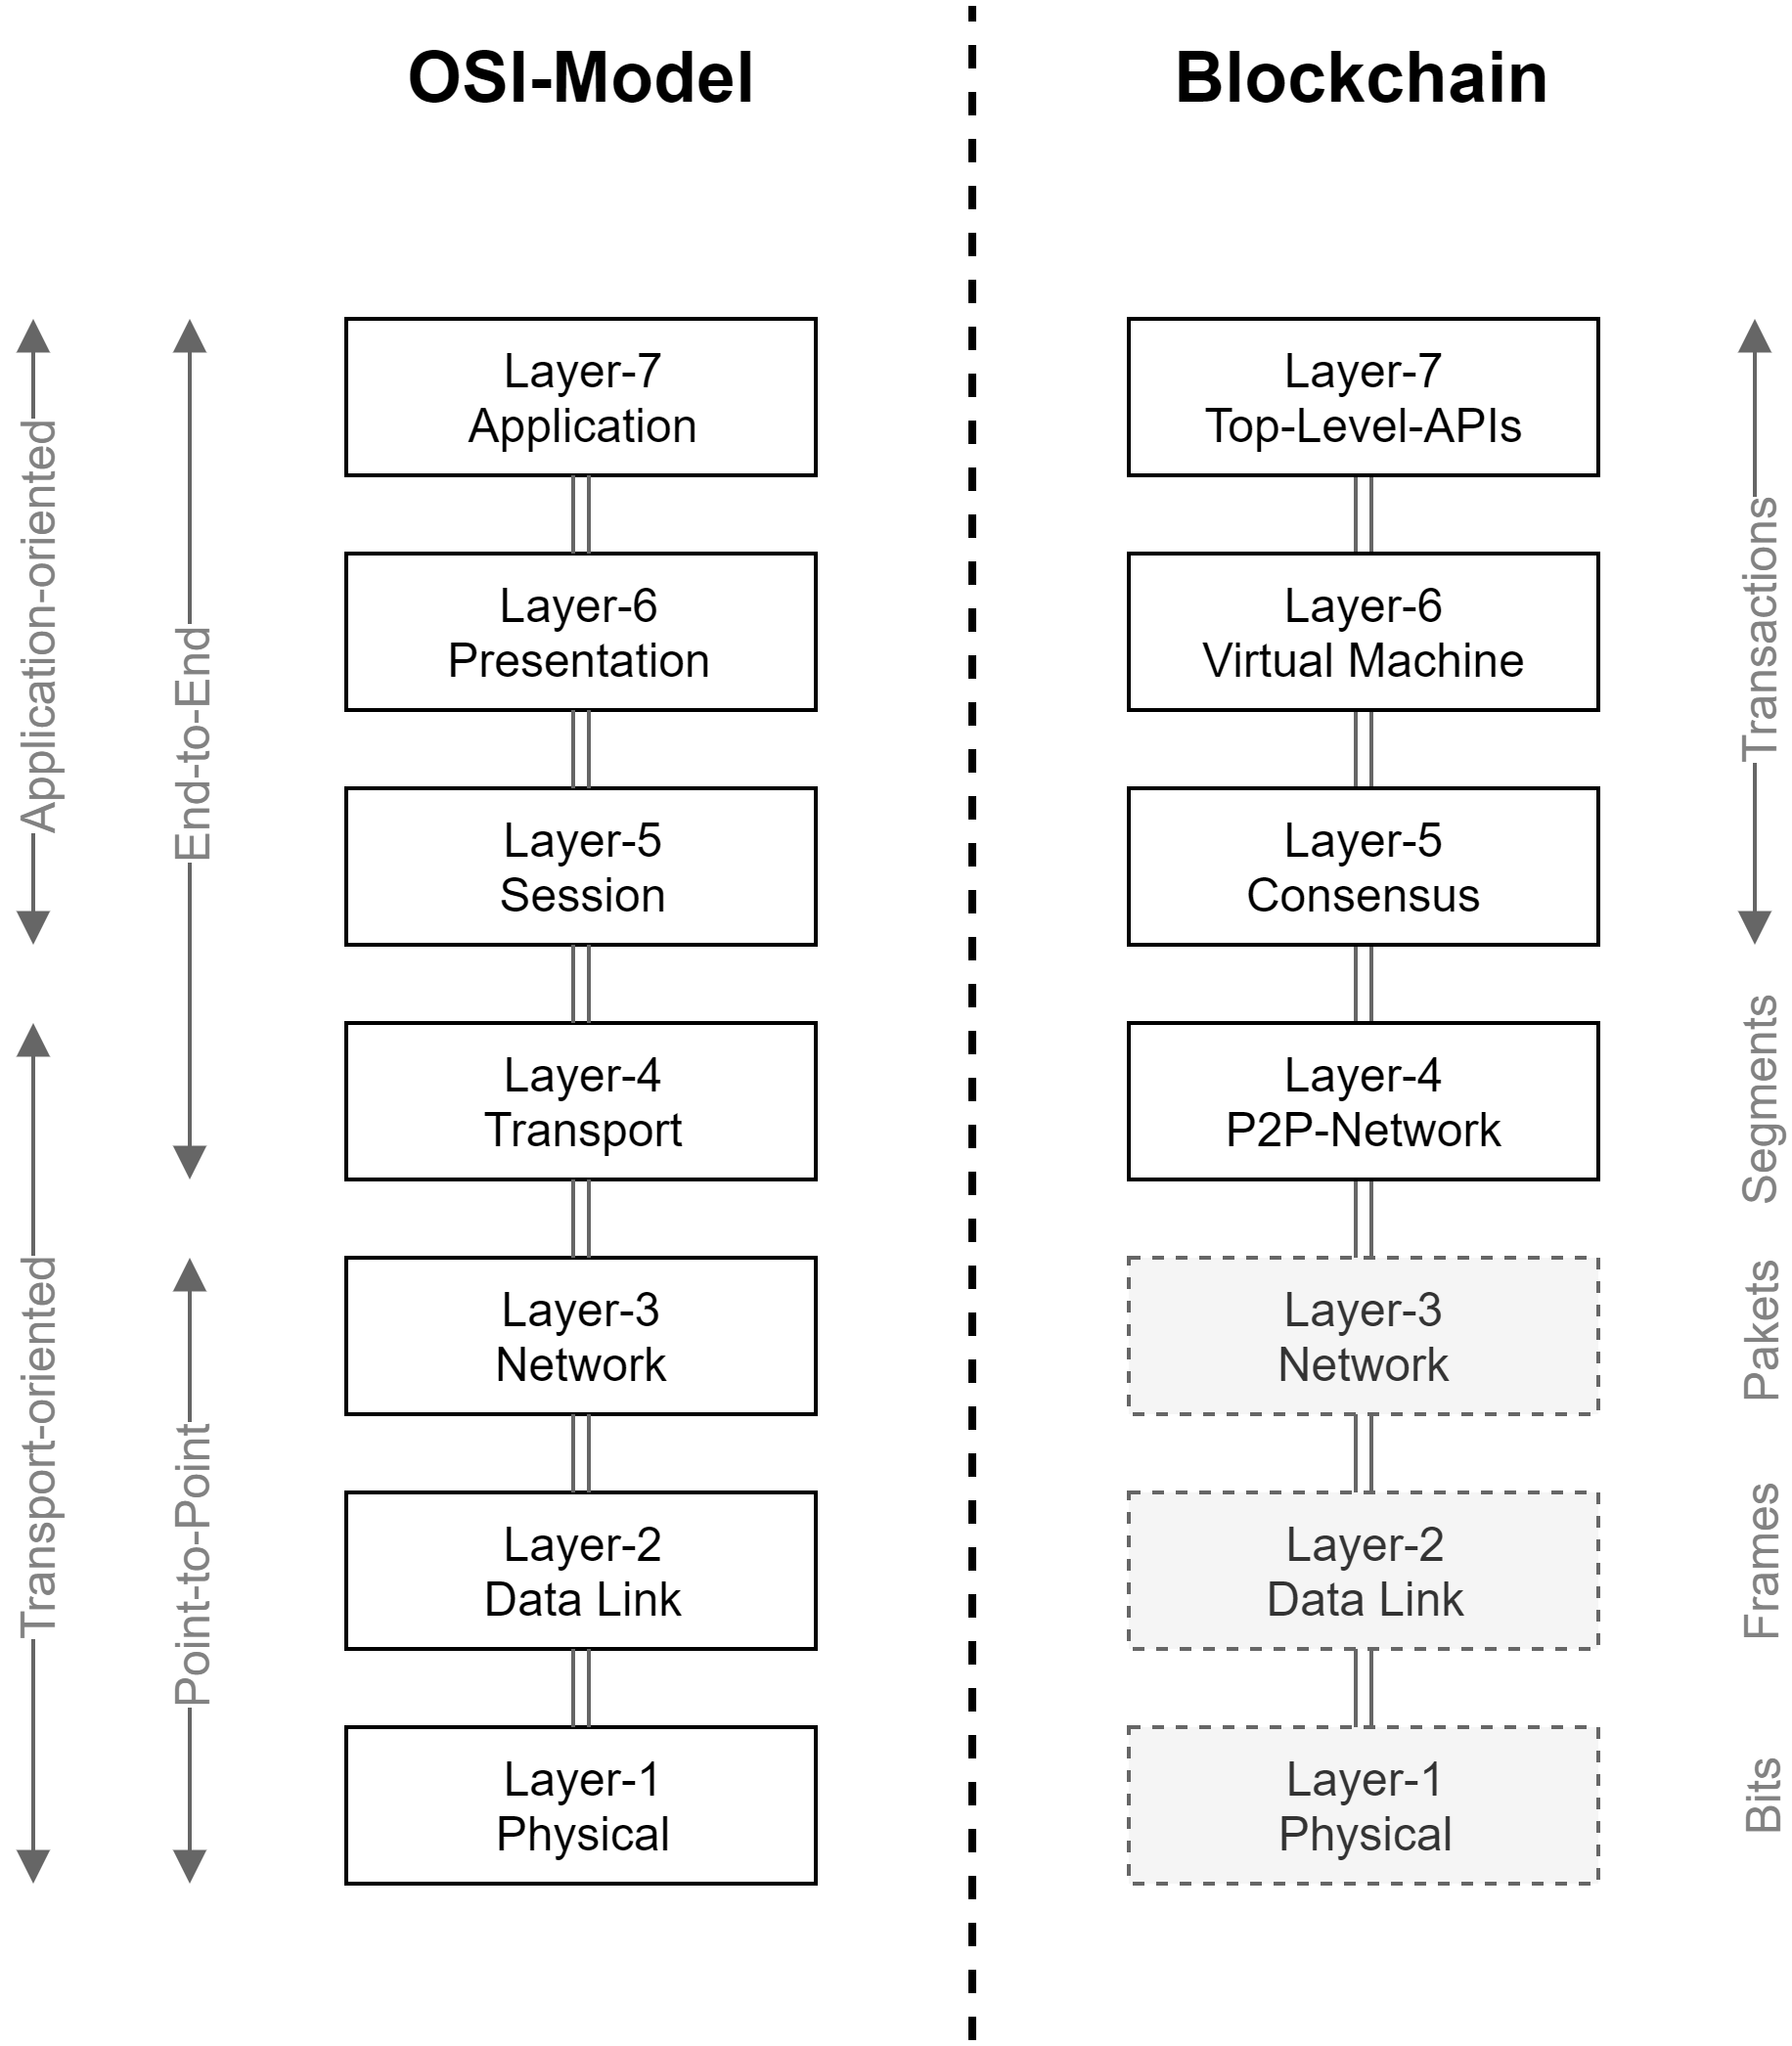
\includegraphics[width=0.7\textwidth]{gfx/osi_blockchain.png}
 \caption{Die Blockchain-Layer im Kontext des OSI-Modells}
 \label{fig:chapter02:osi_blockchain}
\end{figure}

Der Duden \cite{Duden2006} definiert den Begriff Protokoll als \glqq Festlegung von Standards und Konventionen für eine reibungslose Datenübertragung zwischen Computern\grqq. Ein Kommunikationsprotokoll ist gemäß des Gabler Wirtschaftslexikons \cite{Gabler2004} \glqq eine Übermittlungsvorschrift bei der Datenübertragung, die die gesamten Festlegungen für Steuerung und Betrieb der Datenübermittlung in einem Übermittlungsabschnitt [...] umfasst\grqq. Diese Definitionen zusammen mit der Einordnung der Blockchain-Technologie in das \ac{OSI}-Modell suggerieren, dass es sich dabei um ein Kommunikationsprotokoll handelt. Zusammen mit der Zahlungsabwicklung und der Abbildung von Eigentumsverhältnissen beziehungsweise von Eigentumsübergängen spricht man auch von einem sogenannten \glqq Value Exchange Protcol\grqq \cite{bheemaiah2015}.\\
Durch die Einordnung in das \ac{OSI}-Modell kann auch die Sinnfrage beantwortet werden, weshalb die Blockchain-Technologie eine vielversprechende Alternative zu klassischen IT-Systemen darstellt: Betrachtet man die Technologie objektiv, abseits des Hypes und des Anwendungsfalls der Kryptowährungen, so erkennt man eine junge Technologie mit hohem Potenzial. Die Blockchain als Kommunikationsprotokoll gibt dem modernen Softwareentwickler umfangreiche Werkzeuge und Out-of-the-Box Funktionalität über vier Schichten des \ac{OSI}-Modells hinweg an die Hand. Eine dezentrale Plattform mit integrierter Datenbank, Security, Ver- und Entschlüsselung, \ac{P2P}-Netzwerkkommunikation, Entwicklungs- und Laufzeitumgebung für dezentrale Anwendungen, sicherer Zahlungsabwicklung und hoher Verfügbarkeit ist oftmals per Knopfdruck binnen Sekunden erstellt. Alle diese Bestandteile und Funktionalitäten sind in der technischen Spezifikation einer jeden Blockchain in Form eines Kommunikationsprotokolls enthalten und klar definiert.


%
% Section: IOT
%
\section{Internet of Things}
\label{sec:fundamentals:iot}
Der Begriff Internet der Dinge - kurz \ac{IOT} - ist ein Sammelbegriff und bezeichnet die Vernetzung von Gegenständen untereinander (meist über das Internet). Es wird eine autonome \ac{M2M}-Kommunikation ermöglicht, die wiederum den Automatisierungsgrad in dem jeweiligen Einsatzgebiet erhöht. Das bedeutet, dass die Kommunikation zwischen den \ac{IOT}-Geräten selbstständig erfolgt, also ohne das Eingreifen eines Menschen. Nach \cite{deloitte2018} lässt sich das Themenfeld \ac{IOT} in zwei Bereiche untergliedern: \ac{CIOT} und \ac{IIOT}. \ac{CIOT} findet Anwendungen im privaten Umfeld, vor allem geht es hier um Smart-Home und die damit verbundenen Applikationen: Smart-Gardening, Smart-Lights, intelligente Türschließsysteme und Heizungssteuerungen. \ac{IIOT} fokussiert sich auf den kommerziellen Bereich und versucht Anwendungen im deutlich größeren Stil zu entwickeln: Die Bereiche Automotive, Energie und Supply-Chain sind hierbei einige wichtige Vertreter und treten als Smart-Factory, Smart-City, Connected-Cars und Weitere in Erscheinung. Die Abbildung \ref{fig:chapter02:overview-iot} gibt eine Übersicht über die grobe \ac{IOT}-Architektur im Kontext von \ac{DLT}.

\begin{figure}[h]
 \centering
 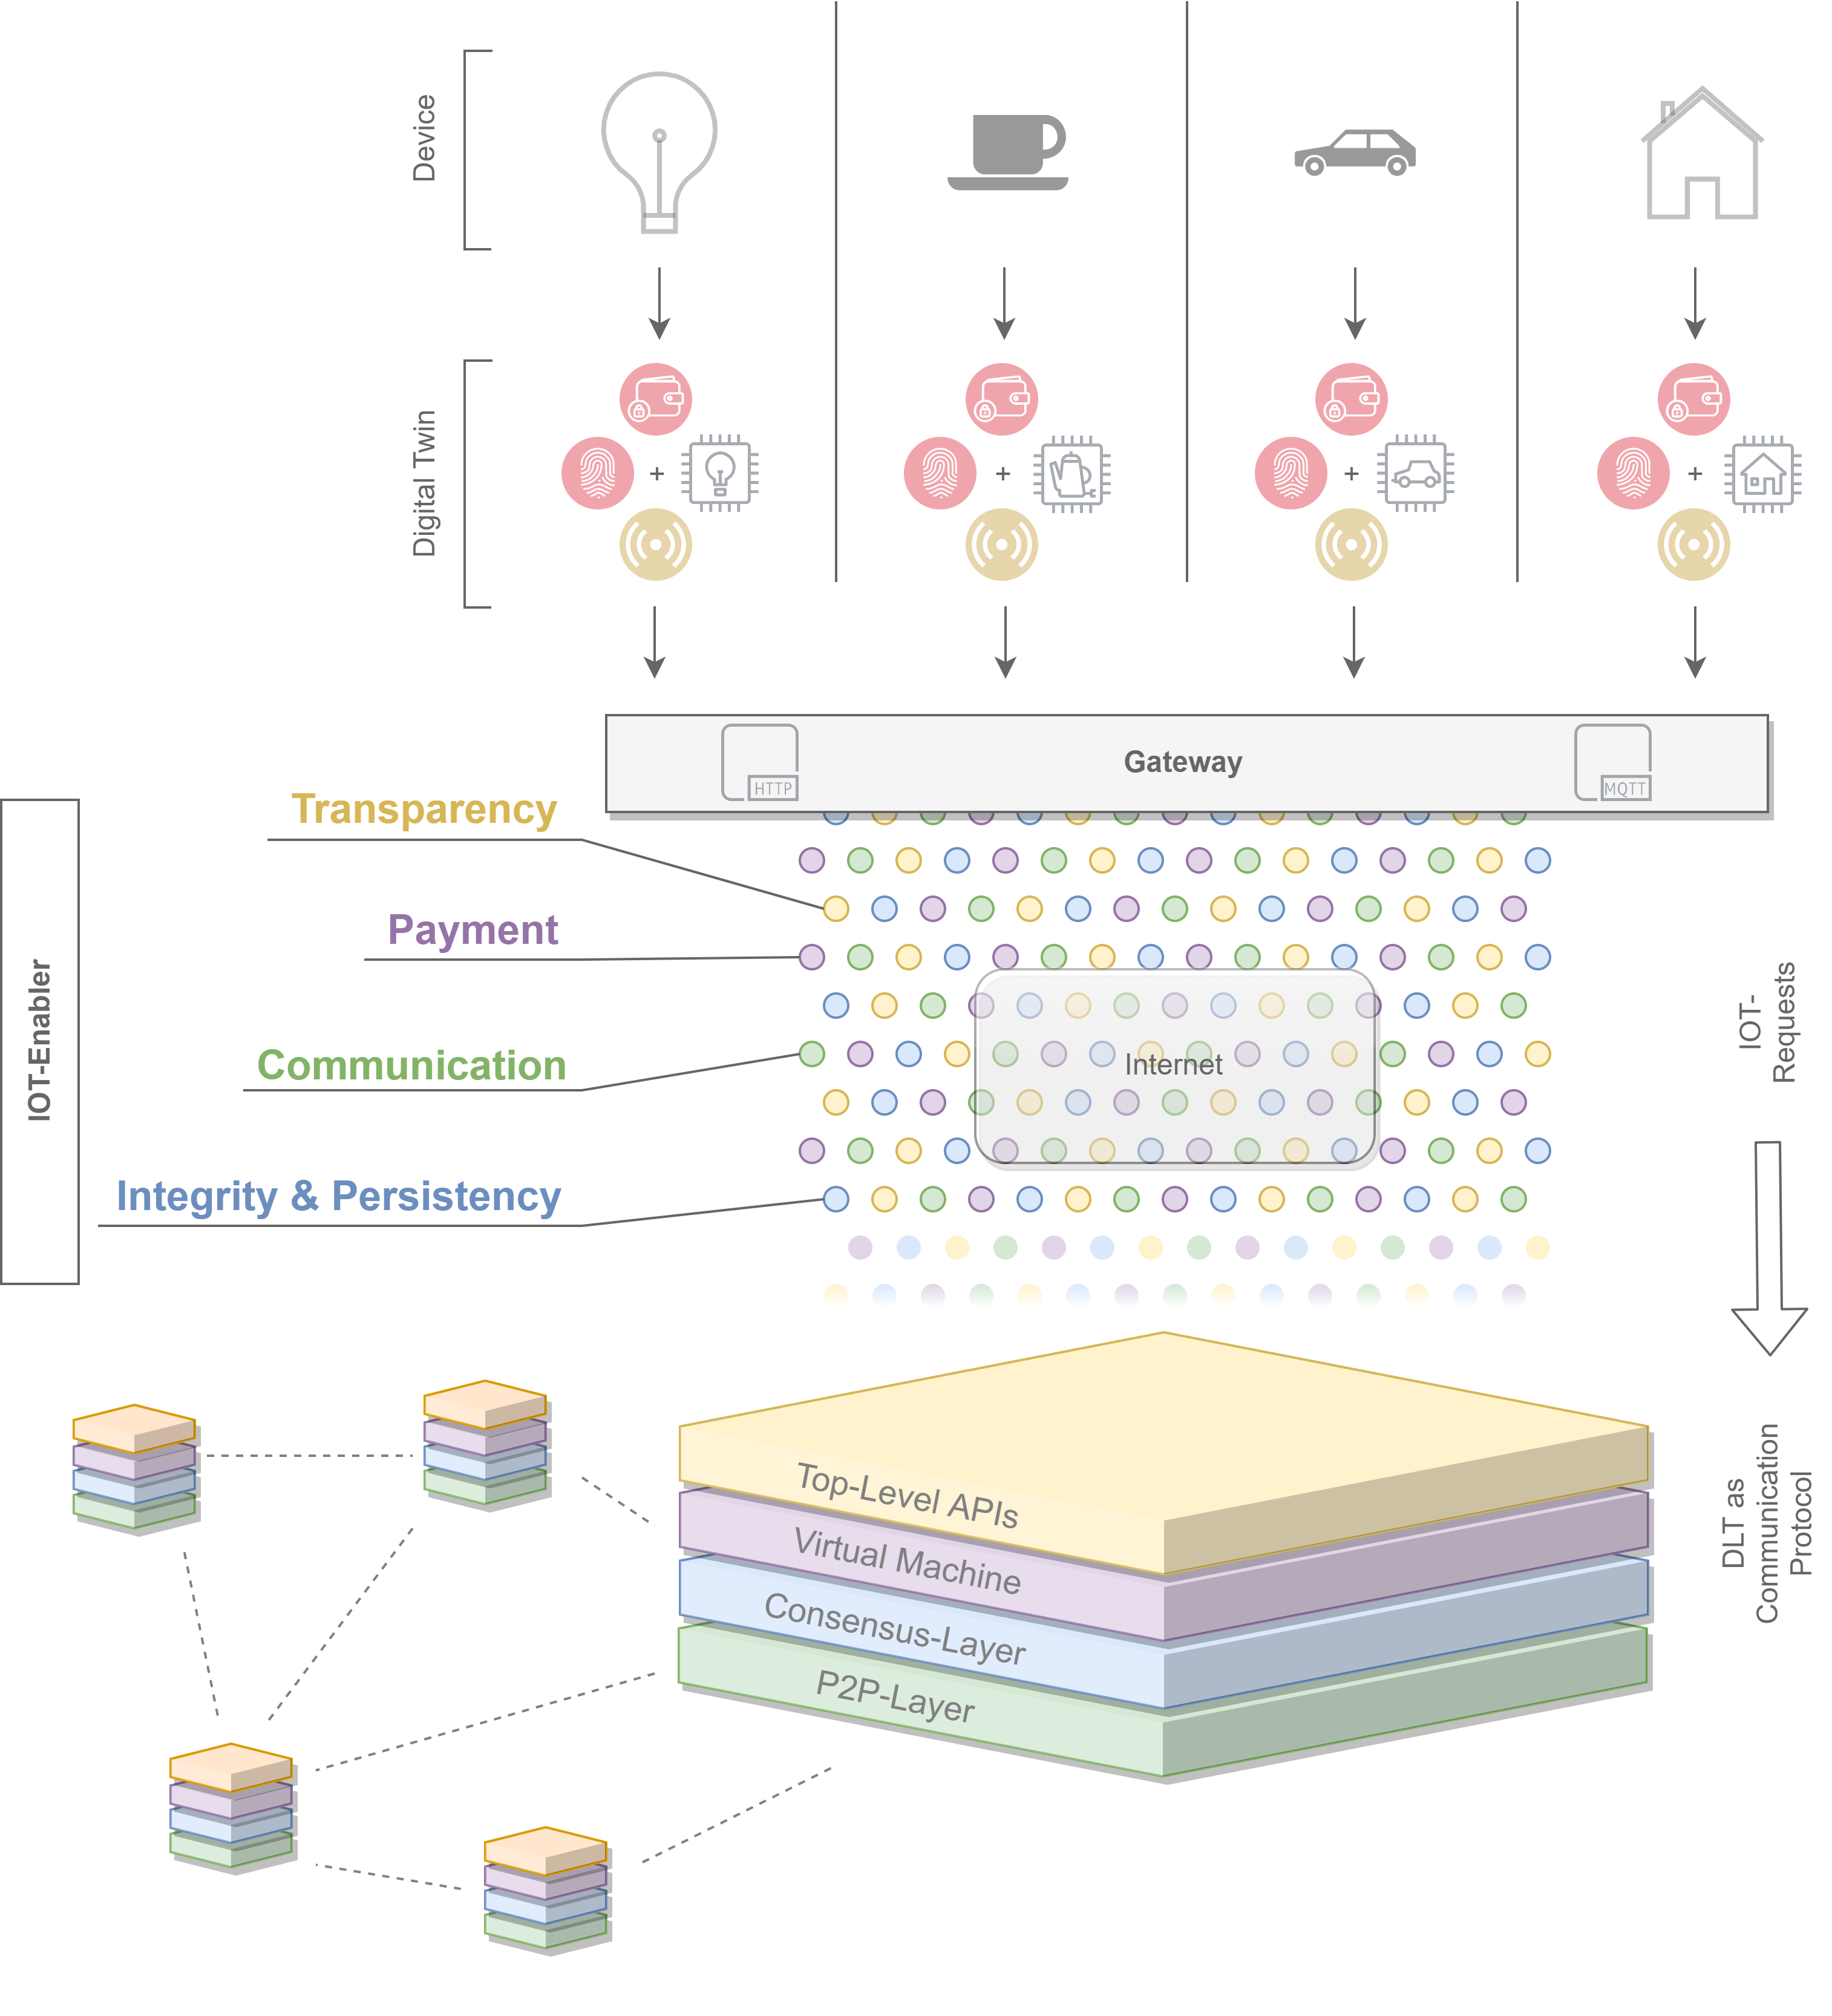
\includegraphics[width=1.0\textwidth]{gfx/Overview-IOT.png}
 \caption{Schematische Darstellung von IOT im Kontext von DLTs}
 \label{fig:chapter02:overview-iot}
\end{figure}

Um physische Geräte miteinander zu vernetzen, werden sogenannte digitale Zwillinge (engl.: Digital Twins) erzeugt. Dabei handelt es sich um virtuelle Abbildungen der Geräte, die mittels Sensoren und Aktoren miteinander verbunden sind. Somit können Zustandsänderungen vom physischen Teil zum virtuellen Teil übertragen werden und umgekehrt. Jedes Gerät besitzt eine eindeutige Identität, die im Blockchain-Umfeld mittels dezentraler Identität abgebildet wird (vgl. \ref{subsec:fundamentals:dlt:did}). Darüber hinaus und abhängig vom Anwendungsfall besitzen Geräte eine Wallet, um automatisierte Bezahlvorgänge \ac{M2M} durchzuführen. Jedes Gerät hat eine bestimmte Funktionalität und trägt einen Teil zum \ac{IOT}-System bei, wobei die Geräte über ein lokales Gateway mit dem Internet verbunden sind; dabei kann es sich beispielsweise um einen WLAN-Router oder einen Mobilfunk-Chip handeln. Die Kommunikation erfolgt über gängige Kommunikationsprotokolle wie MQTT, HTTP oder - wie im Falle von Blockchain - über das Blockchain-Protokoll. \ac{IOT}-Anfragen werden über das Blockchain-Netzwerk prozessiert; aus Sicht eines \ac{IOT} Geräte-Herstellers und Konsumenten formulieren \citeauthor{SCIOT2016} in \cite{SCIOT2016} die Vorteile davon wie folgt:\\
\textit{\glqq From the manufacturer's side, the current centralized model has a high maintenance cost consider the distribution of software updates to millions of devices for years after they have been long discontinued. From the consumer's side, there is a justified lack of a trust in devices that phone home in the background and a need for a security through transparency approach.\grqq}\\
\citeauthor{SCIOT2016} nennen zwei zentrale Kerneigenschaften eines Distributed Ledgers: Zum einen die Verteilung und die einfache Anbindung und Erreichbarkeit von \ac{IOT}-Geräten, die die Wartung seitens des Herstellers erleichtern können. Zum anderen sprechen die Autoren die Vertrauensfrage seitens der Kunden in Bezug auf Datensicherheit und Privatsphäre an. Hier kann die Blockchain-Technologie nach \citeauthor{SCIOT2016} \glqq Sicherheit durch Transparenz\grqq erzielen und für eine größere Akzeptanz sorgen.\\
Der Einsatz von Blockchain-Technologie ist allerdings nicht immer ratsam oder möglich. So kann beispielsweise aufgrund des Anwendungsfalls oder aufgrund von technischen Beschränkungen und Gegebenheiten der Einsatz eines \acp{DLT} im \ac{IOT}-Umfeld unvorteilhaft sein. Ersteres könnte zum Beispiel eine Smart-Home Anwendung sein, die eine Temparaturregelung und Überwachung der eigenen vier Wände vorsieht. Ein dezentraler Ledger wäre hier überdimensioniert und für diesen Zweck überqualifiziert. Der Aufwand stünde in keinem Verhältnis zum Nutzen. Darüber hinaus zeigt dieser \ac{IOT}-Anwendungsfall auch keine Charakteristika einer \ac{DLT}-Anwendung auf: Es handelt sich um eine einzige beteiligte Partei in einem vertrauten Umfeld mit nur wenigen Endgeräten. Auf der anderen Seite können technische Hürden den Einsatz von \ac{DLT} verhindern. Gerade im Automotive-Bereich ist die Verarbeitung von Sensor- und Aktordaten in Echtzeit ein kritischer Punkt. Dezentrale Ledger eigenen sich hierzu nicht, da sie nicht in der Lage sind, zeitkritische Anwendungen zu betreiben.\\
Es wird deutlich, dass die Beschaffenheit des \ac{IOT}-Anwendungsfalls sehr entscheidend dazu beiträgt, ob der Einsatz einer Blockchain-Lösung sinnvoll ist oder nicht. Die Blockchain bietet aufgrund ihrer Kern-Eigenschaften einige IOT-Enabler nativ an: Transparente und überprüfbare Prozesse aller Geräte, integrierte und automatisierte \ac{M2M}-Zahlungsabwicklung, \ac{P2P}-Kommunikation sowie Datenintegrität und -persistenz.

\subsection{Digitaler Zwilling}
\label{subsec:fundamentals:iot:digitaltwins}
Ein digitaler Zwilling (engl. Digital Twin) ist nach \citeauthor{deloitte2018} eine virtuelle Kopie physikalischer Objekte. Digitale Zwillinge werden in automatisierten IT-Prozessen benötigt, da sie als Schnittstelle zwischen physischer Welt und deren digitalen Pendant fungieren. Der Zustand eines physikalischen Objekts wird in den digitalen Zwilling gespiegelt, welcher wiederum eine digitale Zustandsüberwachung und die Manipulation seines physischen Gegenstücks ermöglicht. \cite{deloitte2018}\\
Der Ansatz von digitalen Zwillingen und die Thematik \ac{IOT} haben gegenseitig enormen Einfluss aufeinander und befähigen einander zu neuen Anwendungsfällen. Diese können unter Anderem die Abbildung von Fabriken und Maschinen in digitale Automatisierungsprozesse sein, indem die Geräte und Teile mit Sensoren, Konnektivität und einer Steuerungslogik ausgestattet werden. Dadurch können Predictive Maintance, Bedarfsplanungen und Prozessoptimierungen durchgeführt werden.\\
Im Umfeld Blockchain und \ac{IOT} werden die Begriffe Digital Twin und Dezentrale Identität oft synonym verwendet, da beide ein physikalisches Objekt virtuell abbilden. Dezentralen Identitäten beschreiben als \ac{W3C}-Standard die konkrete Umsetzung, wie virtuelle Identitäten nach der Idee eines Digital Twins standardisiert erzeugt und verwaltet werden können.
